% OOP_intro_beamer.tex
\documentclass[aspectratio=169,11pt]{beamer}

% Theme and appearance (kept standard for portability)
\usetheme{Madrid}
\usecolortheme{default}
\usefonttheme{professionalfonts}

% Packages
\usepackage[utf8]{inputenc}
\usepackage[T1]{fontenc}
\usepackage{lmodern}
\usepackage{amsmath, amssymb}
\usepackage{booktabs}
\usepackage{graphicx}
\usepackage{tikz}
\usetikzlibrary{arrows.meta, positioning, shapes, calc}
\usepackage{listings}
\usepackage{xspace}
\usepackage{hyperref}

% Pseudocode style (no language specified)
\lstdefinelanguage{Pseudo}{
  morekeywords={class,object,interface,abstract,extends,implements,private,public,protected,
  static,virtual,override,final,new,delete,constructor,method,property,field,this,self,return,
  if,else,for,while,foreach,try,catch,finally,throw,raise},
  sensitive=true,
  morecomment=[l]{//},
  morecomment=[s]{/*}{*/},
  morestring=[b]"
}
\lstset{
  language=Pseudo,
  basicstyle=\ttfamily\small,
  keywordstyle=\bfseries,
  commentstyle=\itshape,
  showstringspaces=false,
  frame=single,
  columns=fullflexible,
  keepspaces=true,
  tabsize=2,
  escapeinside={(*}{*)}
}

% Shortcuts
\newcommand{\term}[1]{\textbf{#1}}
\newcommand{\mins}[1]{\textit{(#1 min)}}

% Notes (speaker notes inline)
\setbeameroption{hide notes} % change to show notes on handout if needed
%\setbeameroption{show notes on second screen=right} % for live talk

% Title
\title{An Introduction to Object-Oriented Programming (OOP)}
\subtitle{Concepts, Modeling, Design Principles, and Trade-offs}
\author{Diogo Ribeiro}
\date{\today}

\begin{document}

% ------------------------------------------------------------------
\begin{frame}
  \titlepage
  \note{
    Welcome and context. Emphasize language-agnostic focus. Agenda targets ~90–120 minutes including exercises and Q\&A.
  }
\end{frame}

% ------------------------------------------------------------------
\begin{frame}{Learning Objectives}
  By the end of this session, you will be able to:
  \begin{itemize}
    \item Explain core OOP concepts: objects, classes, identity, state, behavior.
    \item Describe encapsulation, abstraction, inheritance, and polymorphism.
    \item Model simple domains with responsibilities and relationships.
    \item Read and sketch basic class and interaction diagrams.
    \item Apply key design principles (e.g., SOLID) pragmatically.
    \item Recognize trade-offs and common pitfalls in OOP design.
  \end{itemize}
  \note{Set expectations. Note there will be short activities and a brief case study.}
\end{frame}

% ------------------------------------------------------------------
\begin{frame}{Agenda \mins{5}}
  \begin{enumerate}
    \item Why OOP? \mins{10}
    \item Core Concepts \& Terminology \mins{15}
    \item The Four Pillars \mins{25}
    \item Modeling \& Diagrams \mins{15}
    \item Design Principles (SOLID) \mins{15}
    \item Case Study \& Trade-offs \mins{10}
    \item Wrap-up, Quiz, Resources \mins{10}
  \end{enumerate}
  \note{Mention there are two short exercises embedded (~5–7 min each).}
\end{frame}

% =========================
% 1. Why OOP?
% =========================
\section{Why OOP?}

\begin{frame}{Motivation \mins{5}}
  \begin{itemize}
    \item Real-world entities have identity, state, and behavior.
    \item OOP models systems as \term{objects} that interact.
    \item Goals: modularity, reuse, maintainability, and clarity.
    \item Suitable for complex domains with rich interactions.
  \end{itemize}
  \note{Stress mapping from domain concepts to software artifacts.}
\end{frame}

\begin{frame}{When OOP Helps (and When It Doesn’t) \mins{5}}
  \textbf{Helps:}
  \begin{itemize}
    \item Complex domains, evolving requirements.
    \item Teams needing clear ownership and interfaces.
    \item Systems benefiting from composition and extension.
  \end{itemize}
  \vspace{0.5em}
  \textbf{Caution:}
  \begin{itemize}
    \item Over-engineering small scripts.
    \item Deep inheritance hierarchies.
    \item Excessive indirection harming performance/readability.
  \end{itemize}
  \note{Set a balanced tone. OOP is a tool, not a dogma.}
\end{frame}

% =========================
% 2. Core Concepts
% =========================
\section{Core Concepts \& Terminology}

\begin{frame}{Objects and Classes \mins{6}}
  \term{Object}: an entity with identity, state, and behavior.\\[0.4em]
  \term{Class}: a blueprint defining properties (state) and methods (behavior).\\[0.8em]
  \begin{itemize}
    \item \term{Identity}: distinguishes one object from another.
    \item \term{State}: data held by the object (fields/properties).
    \item \term{Behavior}: operations the object can perform (methods).
  \end{itemize}
  \note{Avoid language specifics; keep ideas general.}
\end{frame}

\begin{frame}{Instances, Messages, and Interfaces \mins{4}}
  \begin{itemize}
    \item \term{Instance}: a concrete occurrence of a class.
    \item \term{Message/Call}: a request sent to an object to invoke behavior.
    \item \term{Interface}: a contract describing behavior without revealing implementation.
  \end{itemize}
  \note{Highlight decoupling: clients depend on contracts, not details.}
\end{frame}

\begin{frame}[fragile]{Pseudocode Sketch \mins{5}}
\begin{lstlisting}
// Blueprint
class Counter:
  private value: Integer

  constructor(start: Integer):
    this.value = start

  method increment():
    this.value = this.value + 1

  method read() -> Integer:
    return this.value

// Use
let c = new Counter(0)
c.increment()
print(c.read()) // 1
\end{lstlisting}
\note{Simple, language-agnostic pseudocode to make terms concrete.}
\end{frame}

% =========================
% 3. Four Pillars
% =========================
\section{The Four Pillars}

\begin{frame}{Encapsulation \mins{6}}
  \begin{itemize}
    \item Bundle state and behavior together.
    \item Hide implementation details; expose a stable interface.
    \item Benefits: invariants, safer evolution, reduced coupling.
  \end{itemize}
\end{frame}

\begin{frame}[fragile]{Encapsulation: Example \mins{4}}
\begin{lstlisting}
class BankAccount:
  private balance: Money

  constructor(initial: Money):
    this.balance = initial

  method deposit(amount: Money):
    assert amount > 0
    this.balance = this.balance + amount

  method withdraw(amount: Money):
    assert 0 < amount <= this.balance
    this.balance = this.balance - amount

  method getBalance() -> Money:
    return this.balance
\end{lstlisting}
\note{Only controlled methods can change state; invariant: balance >= 0.}
\end{frame}

\begin{frame}{Abstraction \mins{5}}
  \begin{itemize}
    \item Focus on \emph{what} an object does, not \emph{how}.
    \item Specify behavior via contracts (preconditions, postconditions).
    \item Replaceable implementations behind a stable interface.
  \end{itemize}
\end{frame}

\begin{frame}{Inheritance \mins{5}}
  \begin{itemize}
    \item Mechanism for reusing and specializing behavior.
    \item \term{Subtype} extends or refines a \term{supertype}.
    \item Use with care: prefer composition when reuse is ornamental.
  \end{itemize}
\end{frame}

\begin{frame}{Polymorphism \mins{5}}
  \begin{itemize}
    \item Same message, different implementations.
    \item Enables substitutability and open-ended extension.
    \item Often paired with interfaces/abstract types.
  \end{itemize}
\end{frame}

\begin{frame}[fragile]{Polymorphism: Example \mins{4}}
\begin{lstlisting}
interface Shape:
  method area() -> Number

class Circle implements Shape:
  private r: Number
  method area() -> Number: return 3.14159 * r * r

class Rectangle implements Shape:
  private w: Number; private h: Number
  method area() -> Number: return w * h

// Client code (works with any Shape)
let shapes: List<Shape> = [Circle(2), Rectangle(3,4)]
print(sum(s.area() for s in shapes))
\end{lstlisting}
\note{Client depends on the abstraction, not concrete classes.}
\end{frame}

% =========================
% 4. Modeling & Diagrams
% =========================
\section{Modeling \& Diagrams}

\begin{frame}{From Domain to Design \mins{3}}
  \begin{enumerate}
    \item Identify core domain concepts (nouns) and responsibilities (verbs).
    \item Clarify relationships (association, aggregation, composition).
    \item Define interfaces and collaboration scenarios.
  \end{enumerate}
\end{frame}

\begin{frame}{Basic Class Diagram \mins{6}}
\centering
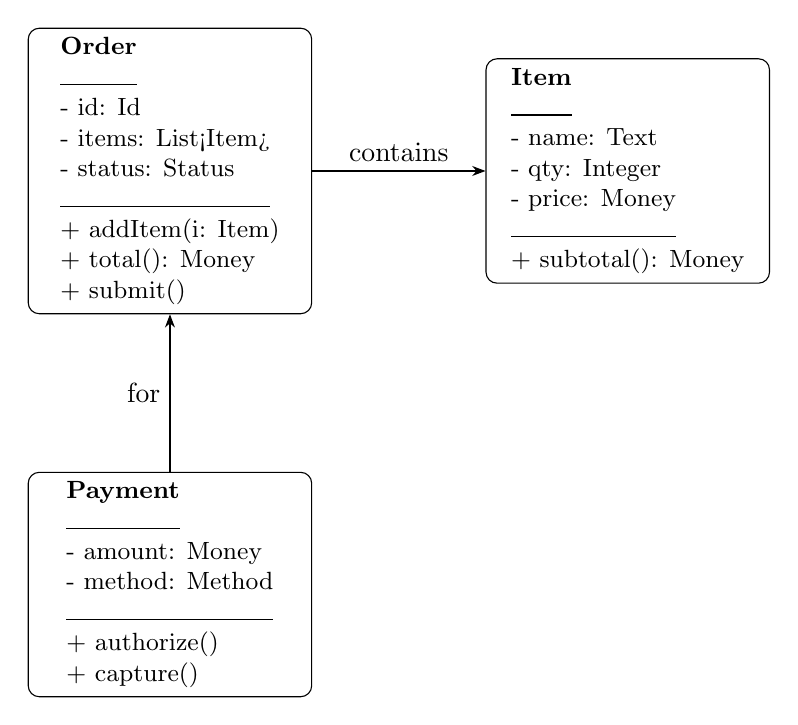
\begin{tikzpicture}[
  class/.style={rectangle, rounded corners, draw, minimum width=3.6cm, align=left, font=\small},
  >={Stealth[length=2.2mm]},
  node distance=2.0cm and 2.2cm
]
\node[class] (Order) { \textbf{Order}\\\hrulefill\\
- id: Id\\- items: List<Item>\\- status: Status\\\hrulefill\\
+ addItem(i: Item)\\+ total(): Money\\+ submit()
};

\node[class, right=of Order] (Item) { \textbf{Item}\\\hrulefill\\
- name: Text\\- qty: Integer\\- price: Money\\\hrulefill\\
+ subtotal(): Money
};

\node[class, below=of Order] (Payment) { \textbf{Payment}\\\hrulefill\\
- amount: Money\\- method: Method\\\hrulefill\\
+ authorize()\\+ capture()
};

\draw[-{Stealth}] (Order) -- node[above]{contains} (Item);
\draw[-{Stealth}] (Payment) -- node[left]{for} (Order);
\end{tikzpicture}
\note{Explain attributes/operations; arrows here are semantic, not strict UML syntax.}
\end{frame}

\begin{frame}{Interaction Sketch (Sequence) \mins{5}}
\begin{itemize}
  \item \textbf{Scenario:} Customer submits an order and pays.
  \item Steps:
  \begin{enumerate}
    \item \texttt{Order.submit()} validates lines, computes total.
    \item \texttt{Payment.authorize()} checks funds.
    \item \texttt{Payment.capture()} finalizes transaction.
  \end{enumerate}
\end{itemize}
\note{Keep it conceptual; focus on message flow, not notation purity.}
\end{frame}

% =========================
% 5. Design Principles
% =========================
\section{Design Principles}

\begin{frame}{SOLID in Practice \mins{10}}
  \begin{itemize}
    \item \textbf{S}: Single Responsibility — one reason to change.
    \item \textbf{O}: Open/Closed — open for extension, closed for modification.
    \item \textbf{L}: Substitution — subtypes must honor supertype contracts.
    \item \textbf{I}: Interface Segregation — many small contracts over one large.
    \item \textbf{D}: Dependency Inversion — depend on abstractions, not details.
  \end{itemize}
  \note{Keep examples language-agnostic; relate back to earlier shapes/order model.}
\end{frame}

\begin{frame}{Composition over Inheritance \mins{5}}
  \begin{itemize}
    \item Prefer assembling behavior from parts to rigid hierarchies.
    \item Reduces coupling and diamond problems.
    \item Inheritance still useful for true “is-a” relationships.
  \end{itemize}
\end{frame}

\begin{frame}{Law of Demeter \mins{3}}
  \begin{itemize}
    \item Talk only to your immediate collaborators.
    \item Avoid “train wreck” calls (chained navigation across objects).
  \end{itemize}
\end{frame}

% =========================
% 6. Activity 1
% =========================
\section{Activity: Object Discovery}

\begin{frame}{Activity 1: Identify Objects \& Responsibilities \mins{7}}
  \textbf{Prompt:} Choose a simple domain (library loans, food delivery, or ticket booking).\\[0.6em]
  \textbf{Task:}
  \begin{enumerate}
    \item List candidate objects, their state, and responsibilities.
    \item Propose 2–3 interactions among them.
  \end{enumerate}
  \textbf{Deliverable:} A quick sketch on paper or whiteboard.
  \note{Timebox to 5 minutes + 2 minutes share-out.}
\end{frame}

% =========================
% 7. Case Study & Trade-offs
% =========================
\section{Case Study \& Trade-offs}

\begin{frame}[fragile]{Case Study: Payment Methods \mins{8}}
\begin{lstlisting}
interface PaymentMethod:
  method authorize(amount: Money) -> Boolean
  method capture(amount: Money) -> Boolean

class CardPayment implements PaymentMethod:
  method authorize(amount): /* talks to card network */ return true
  method capture(amount):   /* settle */ return true

class WalletPayment implements PaymentMethod:
  method authorize(amount): /* wallet API */ return true
  method capture(amount):   /* settle */ return true

class Checkout:
  method pay(orderTotal: Money, pm: PaymentMethod):
    require orderTotal > 0
    if pm.authorize(orderTotal):
      return pm.capture(orderTotal)
    else:
      return false
\end{lstlisting}
\note{Discuss substitutability, testability, and extension with a new method (e.g., voucher).}
\end{frame}

\begin{frame}{Trade-offs \mins{6}}
  \begin{itemize}
    \item \textbf{Flexibility vs. Simplicity}: Abstractions add indirection.
    \item \textbf{Reuse vs. Performance}: Extra dispatch or object hops may cost.
    \item \textbf{Inheritance vs. Composition}: Maintainable extension paths.
    \item \textbf{Granularity}: Over-segmentation leads to “class explosion”.
  \end{itemize}
\end{frame}

% =========================
% 8. Activity 2
% =========================
\section{Activity: Improve a Design}

\begin{frame}{Activity 2: Refactor Toward SOLID \mins{7}}
  \textbf{Prompt:} A \texttt{ReportGenerator} both fetches data, formats it, and writes files.\\
  \textbf{Task:} Split responsibilities and introduce abstractions where helpful.
  \begin{itemize}
    \item Identify at least 2 interfaces.
    \item Show how a new output format would be added without modifying existing code.
  \end{itemize}
  \note{Timebox to 5 minutes + 2 minutes share-out.}
\end{frame}

% =========================
% 9. Testing & Contracts
% =========================
\section{Testing \& Contracts}

\begin{frame}{Design by Contract \mins{5}}
  \begin{itemize}
    \item \term{Preconditions}: what must be true before a call.
    \item \term{Postconditions}: what is guaranteed after a call.
    \item \term{Invariants}: what remains true for a class’s state.
  \end{itemize}
\end{frame}

\begin{frame}{Substitutability (LSP) Checks \mins{5}}
  \begin{itemize}
    \item Subtypes must not strengthen preconditions nor weaken postconditions.
    \item Clients should not need to know the concrete type.
    \item Violations often surface as surprising runtime behavior.
  \end{itemize}
\end{frame}

% =========================
% 10. Patterns (Optional Taste)
% =========================
\section{A Taste of Patterns}

\begin{frame}{Why Patterns? \mins{5}}
  \begin{itemize}
    \item Shared vocabulary for recurring design problems.
    \item Examples: Strategy, Adapter, Composite, Observer, Factory.
    \item Use judiciously; avoid pattern-driven overdesign.
  \end{itemize}
\end{frame}

\begin{frame}[fragile]{Example: Strategy \mins{5}}
\begin{lstlisting}
interface PricingRule:
  method price(order: Order) -> Money

class RegularPricing implements PricingRule:
  method price(order): return order.total()

class HolidayDiscount implements PricingRule:
  method price(order): return order.total() * 0.9

class Checkout:
  private rule: PricingRule
  constructor(rule): this.rule = rule
  method finalPrice(order): return this.rule.price(order)
\end{lstlisting}
\note{Swap behaviors at runtime; open for new rules without modifying Checkout.}
\end{frame}

% =========================
% 11. Pitfalls & Heuristics
% =========================
\section{Pitfalls \& Heuristics}

\begin{frame}{Common Pitfalls \mins{6}}
  \begin{itemize}
    \item God objects and feature envy.
    \item Overuse of inheritance; fragile base classes.
    \item Anemic domain models (data holders with no behavior).
    \item Leaky abstractions and tight coupling.
  \end{itemize}
\end{frame}

\begin{frame}{Heuristics \mins{4}}
  \begin{itemize}
    \item Name classes by responsibility, not by data container role.
    \item One clear reason to change.
    \item Prefer small, cohesive interfaces.
    \item Make illegal states unrepresentable.
  \end{itemize}
\end{frame}

% =========================
% 12. Quick Quiz & Wrap-up
% =========================
\section{Wrap-up}

\begin{frame}{Quick Quiz \mins{6}}
  \begin{enumerate}
    \item What are the four pillars of OOP?
    \item Why is composition often preferred over inheritance?
    \item Give a brief example of polymorphism.
    \item What makes a good interface?
  \end{enumerate}
\end{frame}

\begin{frame}{Key Takeaways \mins{3}}
  \begin{itemize}
    \item Think in terms of responsibilities and collaborations.
    \item Encapsulation and abstraction reduce coupling.
    \item Use inheritance sparingly; embrace polymorphism via interfaces.
    \item Apply principles pragmatically; measure outcomes.
  \end{itemize}
\end{frame}

\begin{frame}{Further Exploration \mins{2}}
  \begin{itemize}
    \item Practice modeling small domains weekly.
    \item Rewrite a procedural solution into object collaborations.
    \item Study a few design patterns; implement tiny examples.
  \end{itemize}
\end{frame}

% =========================
% Appendix
% =========================
\appendix

\begin{frame}{Appendix: Glossary}
\begin{tabular}{@{}ll@{}}
\toprule
Term & Meaning \\
\midrule
Object & Entity with identity, state, behavior \\
Class & Blueprint for objects \\
Interface & Contract describing behavior \\
Encapsulation & Hiding representation behind methods \\
Abstraction & Focus on intent, not implementation \\
Polymorphism & One interface, many forms \\
Inheritance & Reuse/extension via subtype \\
\bottomrule
\end{tabular}
\end{frame}

\begin{frame}{Appendix: Relationship Types}
  \begin{itemize}
    \item \textbf{Association}: “uses/knows about”.
    \item \textbf{Aggregation}: whole–part, parts may exist independently.
    \item \textbf{Composition}: strong ownership; parts’ lifecycle bound to whole.
    \item \textbf{Dependency}: relies on behavior of another type.
  \end{itemize}
\end{frame}

\begin{frame}{Appendix: Timing Plan (90–120 min)}
\small
\begin{tabular}{@{}ll@{}}
\toprule
Segment & Minutes \\
\midrule
Intro, Objectives, Agenda & 5 \\
Why OOP? & 10 \\
Core Concepts & 15 \\
Four Pillars & 25 \\
Modeling \& Diagrams & 15 \\
Activity 1 & 7 \\
Design Principles & 15 \\
Case Study \& Trade-offs & 10 \\
Activity 2 & 7 \\
Quiz, Wrap-up & 6 \\
Buffer / Q\&A & 5--15 \\
\bottomrule
\end{tabular}
\note{Adjust in real time; use buffer for questions or deeper dives.}
\end{frame}

\begin{frame}[plain]
  \centering
  \Huge Thank you!
\end{frame}

\end{document}
